%% pandoc-linguexx -- the manual.
%%
%% Build with LuaLaTeX:   make manual     (or: cd docs/manual && lualatex pandoc-linguexx)
%%
%% The figures are real conversions, laid out by LibreOffice and cropped:
%% figures/make-figures.sh regenerates them from figures/src/.  They are
%% committed, so building the manual needs neither pandoc nor LibreOffice.
%%
%% Copyright (C) 2026 Gerhard Schaden.  Licensed like the program, GPL-3.0
%% or later.
\documentclass[11pt,a4paper]{article}
\usepackage{iftex}
\ifPDFTeX
  \PackageError{pandoc-linguexx}{Build this manual with lualatex}
    {It quotes Unicode (the math asterisk, visible spaces, accented
     names) that pdfLaTeX would need a font setup for.}
\fi
\usepackage[margin=30mm]{geometry}
\usepackage{microtype}
\usepackage{xcolor}
\usepackage{array}
\usepackage{booktabs}
\usepackage{longtable}
\usepackage{tabularx}
\usepackage{enumitem}
\usepackage{fancyvrb}
\usepackage{graphicx}
\usepackage{caption}
\usepackage[lazy]{linguexx}
\usepackage[colorlinks,linkcolor=blue!50!black,urlcolor=blue!50!black]{hyperref}

\emergencystretch=3em

% --- documentation helpers (as in the linguexx manual) ----------------------
\newcommand{\cs}[1]{\texttt{\textbackslash #1}}
\newcommand{\opt}[1]{\texttt{#1}}
\newcommand{\file}[1]{\texttt{#1}}
\newcommand{\sty}[1]{\textsf{#1}}
\newcommand{\meta}[1]{\textrm{\itshape\textlangle#1\textrangle}}
\newcommand{\menu}[1]{\textsf{#1}}
\newcommand{\prog}[1]{\textsf{#1}}
\newcommand{\pkg}[1]{\textsf{#1}}
\DefineVerbatimEnvironment{code}{Verbatim}
  {frame=leftline,framerule=1pt,rulecolor=\color{gray!40},
   xleftmargin=8pt,fontsize=\small}
\newenvironment{note}
  {\par\smallskip\noindent\begin{minipage}{\linewidth}\small\textbf{Note.}\ }
  {\end{minipage}\par\smallskip}

\captionsetup{font=small,labelfont=bf}

\title{\textbf{pandoc-linguexx}\\[4pt]
  \large Converting linguexx documents to LibreOffice Writer and Word}
\author{Gerhard Schaden}
\date{Version 0.1.0 \quad\textbullet\quad targets linguexx~1.4\\ October 2026}

\begin{document}
\maketitle

\begin{abstract}\noindent
\prog{pandoc-linguexx} converts a \LaTeX{} document written with
\pkg{linguexx} into a LibreOffice Writer (\file{.odt}) or Word (\file{.docx})
file in which every example number is a live field. Insert an example in
the word processor and everything after it renumbers, cross-references
included. The rest of the document --- sections, prose, footnotes, tables,
citations --- goes through pandoc, and the converter finishes what pandoc
leaves undone: numbered headings, captions and equations, and
cross-references to all of them, live fields wherever the word processor
allows. The project also contains a Writer macro
and Word and OnlyOffice add-ins that build the same examples inside the
word processor, and a converter for the way back to \LaTeX.
\end{abstract}

\tableofcontents

% ============================================================================
\section{Introduction}

A linguist who writes in \LaTeX{} with \pkg{linguexx} sooner or later has to
hand a paper to someone who works in a word processor: a co-author, an
editor, a journal that accepts only \file{.docx}. Pandoc converts the prose
well, but it knows nothing of glossed examples: the alignment of words and
glosses is lost, and the example numbers become plain text that no longer
follows when an example is added.

\prog{pandoc-linguexx} keeps both. Each example becomes a borderless table
whose columns align the object language with its glosses, and each number is
a field --- a \emph{number range} field in Writer, a \texttt{SEQ} field in
Word --- so that the word processor renumbers. References to examples are
fields pointing at those numbers.

The project has three parts, which share one specification:
\begin{description}[style=nextline,leftmargin=1.5em]
\item[\prog{linguexx2odt}] the converter: \LaTeX{} to \file{.odt} or
  \file{.docx}. Most of this manual is about it.
\item[The Writer macro and the Word and OnlyOffice add-ins] build the same
  examples inside the word processor from a few typed lines, so that a
  converted document can be extended in kind (section~\ref{sec:inside}).
\item[\prog{docx2linguexx} and \prog{odt2linguexx}] take a document edited
  in the word processor back to \LaTeX{} (section~\ref{sec:back}).
\end{description}

Four principles run through all of it:
\begin{enumerate}
\item \textbf{Numbers are live.} An example number, a section number, a
  caption's number and every reference to them is a field the word processor
  recomputes. Where that is not possible, the manual says so.
\item \textbf{Nothing is direct formatting.} Every paragraph and character
  the converter writes carries a named style (\sty{LxExampleCell},
  \sty{LxLeipzig}, \ldots), so a whole document is restyled from the style
  list.
\item \textbf{\LaTeX{} is the reference.} What a reference, a caption or a
  number prints is not reasoned out: it was measured from what \LaTeX{}
  prints for the same source, and the test suite holds the converter to it.
\item \textbf{It never fails silently.} Anything it cannot render
  faithfully is named in a warning. Some constructs degrade, a few are
  deleted; section~\ref{sec:limits} lists them.
\end{enumerate}

\begin{note}
The \file{.odt} target is the reference one: it is what the Writer macro is
built against. The \file{.docx} target writes the same examples, fields and
styles, and reads correctly in Word~365, LibreOffice and OnlyOffice.
\end{note}

% ============================================================================
\section{Installation}\label{sec:install}

\subsection{Requirements}

\begin{center}
\begin{tabular}{@{}l l p{6.6cm}@{}}
\toprule
\textbf{Program} & \textbf{Version} & \textbf{Needed for}\\
\midrule
pandoc & 3.0 or later & every conversion; tested with 3.6.1 and 3.10.2\\
Python & 3.10 or later & the converter itself\\
\texttt{fonttools} & any & measuring a face other than Times (installed with the package)\\
\midrule
LibreOffice & optional & the page numbers of \cs{pageref} (section~\ref{sec:pages}),
  \prog{odt2linguexx}, the test suite\\
\texttt{pdfinfo} (poppler) & optional & the page numbers, with LibreOffice\\
\texttt{kpsewhich} (\TeX{}) & optional & finding files \cs{input} names through \texttt{TEXINPUTS}\\
\bottomrule
\end{tabular}
\end{center}

LibreOffice is \emph{not} needed to convert. It is only needed to read the
result, to fill in page numbers ahead of time, and to run the half of the test
suite that renders documents.

\subsection{Installing}

The package installs the three commands \prog{linguexx2odt},
\prog{docx2linguexx} and \prog{odt2linguexx}. With \prog{pipx}, the
command lands on the \texttt{PATH} by itself:
\begin{code}
pipx install -e /path/to/pandoc-linguexx
\end{code}
Many current distributions refuse \texttt{pip install} into the system Python.
Use a virtual environment instead:
\begin{code}
python -m venv .venv
.venv/bin/pip install -e .
.venv/bin/linguexx2odt paper.tex
\end{code}
Or install nothing, and run it from a checkout:
\begin{code}
PYTHONPATH=src python3 -m linguexx2odt paper.tex
\end{code}
The \texttt{PYTHONPATH} is not optional there: the project uses a \texttt{src}
layout, so a bare \texttt{python3 -m linguexx2odt} in the repository's root
does not find the package.

% ============================================================================
\section{Quick start}\label{sec:quick}

\begin{code}
linguexx2odt paper.tex                    # writes paper.odt
linguexx2odt paper.tex --to docx          # writes paper.docx
linguexx2odt paper.tex -o draft.odt -v    # another name; report what was done
\end{code}

The run prints a warning for anything it could not render faithfully, with
the line it is about. Read them: they are the list of what to check in the
output.

Figure~\ref{fig:gloss} shows three examples as \pkg{linguexx} sets them and as
the converter writes them. The source is the same, given below the figure.

\begin{figure}[htbp]
\textbf{\small\LaTeX{} with linguexx}\par\medskip
\setcounter{ExNo}{0}
\ex. The cat is on the mat.

\ex. \a. \gll Le chat dort\\
                 the cat sleeps\\
     \glt `The cat sleeps.'
\b. * \gll Chat le dort\\
           cat the sleeps\\
     \glt `The cat sleeps.'

\ex. \gll Hans hat \lpzg{dem} Kind {ein Buch} gegeben\\
          Hans has the.\lpzg{dat} child a book given\\
\glt `Hans gave the child a book.'

\medskip
\textbf{\small Converted to \file{.odt}, as LibreOffice lays it out}\par\medskip
\noindent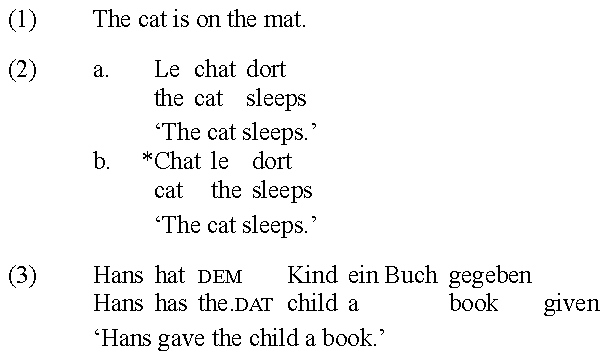
\includegraphics{figures/gloss-odt}
\caption{The same source set by \LaTeX{} (above) and converted to
\file{.odt} (below). Numbers, sub-example letters, the judgment hanging to
the left, glosses under their words and \texttt{\{ein Buch\}} as one
column all survive.}
\label{fig:gloss}
\end{figure}

\VerbatimInput[frame=leftline,framerule=1pt,rulecolor=\color{gray!40},
  xleftmargin=8pt,fontsize=\small,firstline=4,lastline=15]{figures/src/gloss.tex}

To check that the numbers are live: in Writer, put the cursor before an
example, insert a new number field (\menu{Insert \textrightarrow{} Field
\textrightarrow{} More Fields \textrightarrow{} Variables \textrightarrow{}
Number range}, \texttt{NumEx}), then update the fields
(\menu{Tools \textrightarrow{} Update \textrightarrow{} Fields}, or
\texttt{F9}). Every later number and every reference shifts. The Writer macro
(section~\ref{sec:inside}) does this for you, building the whole example
around the number.

% ============================================================================
\section{The command line}\label{sec:cli}

\begin{code}
linguexx2odt [options] input.tex
\end{code}

\begin{longtable}{@{}>{\ttfamily}p{4.1cm} p{9.5cm}@{}}
\toprule
\normalfont\textbf{Option} & \textbf{Effect}\\
\midrule
\endhead
\multicolumn{2}{@{}l}{\emph{Output}}\\[2pt]
-o, --output \meta{file} & The output file. Default: the input's name with
  the target's extension.\\
--to odt|docx & The target format. Default: \texttt{odt}.\\
--reference-doc \meta{file} & A pandoc reference document supplying the base
  styles. It also fixes the face (\opt{--font} is then ignored). Its heading
  numbering is replaced by the converter's (section~\ref{sec:sections}).\\
--page a4|a4-wide|letter|keep & The page geometry written into the
  \file{.odt}. Default: \texttt{a4}; \texttt{keep} leaves pandoc's US Letter.\\[4pt]
\multicolumn{2}{@{}l}{\emph{Layout of the examples}}\\[2pt]
--text-width \meta{cm} & The width of the text block the columns are
  computed for. Default: 17 (A4 with 2\,cm margins).\\
--font \meta{name} & The face the document is set in and its columns are
  measured for. Default: Times New Roman (section~\ref{sec:widths}).\\
--font-pt \meta{pt} & The body size assumed for the measurements. Default: 12.\\
--no-split & Do not break a glossed example too wide for the block into
  bands; squeeze it into one instead (section~\ref{sec:bands}).\\
--example-spacing \meta{cm} & The space above and below each example.
  Default: 0.18. Afterwards it is the style \sty{LxExampleSpace}.\\
--space-above \meta{cm}, --space-below \meta{cm} & Override it above or below only
  (styles \sty{LxExampleSpaceAbove}, \sty{LxExampleSpaceBelow}).\\[4pt]
\multicolumn{2}{@{}l}{\emph{Citations}}\\[2pt]
--bibliography \meta{file.bib} & A bibliography to resolve citations
  against; repeatable. Default: those the document names with
  \cs{addbibresource} or \cs{bibliography}.\\
--csl \meta{style} & A CSL style. Default: pandoc's Chicago author--date,
  which reads like natbib's author--year mode.\\
--no-citeproc & Do not resolve citations; print their keys.\\[4pt]
\multicolumn{2}{@{}l}{\emph{Diagnostics}}\\[2pt]
-q, --quiet & Suppress the warnings.\\
-v, --verbose & Report what was converted.\\
--keep-intermediates \meta{dir} & Keep the intermediate files: the
  residue pandoc reads, its AST, the file before post-processing.\\
--print-macro & Print the Writer macro's source and exit.\\
\bottomrule
\end{longtable}

% ============================================================================
\section{Examples}\label{sec:examples}

\subsection{What is converted}

The converter reads \pkg{linguexx}'s \emph{lazy} syntax, which is
\pkg{linguex}'s:
\begin{itemize}[nosep]
\item \cs{ex.}, sub-examples \cs{a.}, \cs{b.}, \ldots{} on two levels
  (letters, then roman numerals), \cs{z.} to end a level early;
\item glosses: \cs{gll}, \cs{glll}, \cs{gl}\,\ldots\,\cs{endgl}, the
  translation \cs{glt}, the shorthands \cs{exg.}, \cs{ag.}, \cs{bg.};
\item \texttt{\{braced groups\}} as one column, tiers of unequal length;
\item judgments (\texttt{*}, \texttt{??}, \cs{\#}, \cs{jdg}\{\ldots\});
\item \cs{label}, \cs{sublabel}, \cs{ref}, \cs{pref}, \cs{cref}, the relative
  references \cs{Next}, \cs{Last}, \cs{NNext}, \cs{LLast}, ranges
  \cs{refrange} and \cs{prefrange} (section~\ref{sec:xref});
\item \cs{lpzg}\{\ldots\} for Leipzig gloss labels, in small capitals;
\item the brackets \cs{ExLBr}/\cs{ExRBr}, the counters \cs{Exalph} and
  \cs{Exroman}, structural labels \cs{exannot}\{\ldots\} in a column at
  0.75 of the text block, as \cs{ExAnnotColumn} puts them;
\item custom labels \cs{ex.[(4')]}, printed as they are, and inline verbatim
  (\cs{verb}, \cs{Verb}, \cs{lstinline});
\item footnotes inside an example, and the document's own macros, which are
  expanded.
\end{itemize}

An example ends where \pkg{linguexx} ends it: at a blank line, at \cs{z.},
at an environment boundary or at a closing brace.

\subsection{How an example is laid out}

Each example is one borderless table, so its columns line up:
\begin{itemize}
\item The number is a field (\texttt{NumEx} in both formats) between
  literal brackets: the brackets are the document's, \cs{ExLBr} and
  \cs{ExRBr}.
\item Each object-language word sits in a cell of its own, with its glosses
  in the cells below it. The free translation spans the last row.
\item A judgment mark \emph{hangs} to the left of the text, in a column cut
  out of the one before it. A judged and an unjudged example therefore begin
  at the same place, as in \pkg{linguexx}, and a sub-example's letter sits
  where a main example's text begins.
\item A paradigm of sub-examples shares one table, but each item is measured
  on its own words: the table's columns are the union of every boundary
  its items need.
\end{itemize}

\subsection{Long examples: bands}\label{sec:bands}

A glossed example too wide for the text block is split into \emph{bands}:
groups of tier rows, each starting again at the left margin
(figure~\ref{fig:bands}). The number appears on the first band only and the
translation once, at the end. With \opt{--no-split} the example is squeezed
into a single band instead, its words wrapping inside their cells.

\begin{figure}[htbp]
\centering
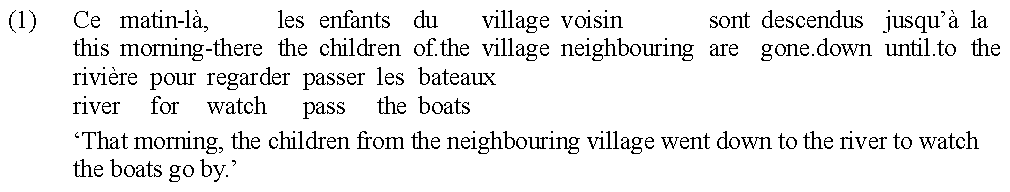
\includegraphics[width=\linewidth]{figures/bands-odt}
\caption{A glossed example too wide for the text block, split into two
bands. Each band starts again at the left; the translation comes once.}
\label{fig:bands}
\end{figure}

A word processor's table does not reflow. The break points are computed at
conversion time from \opt{--text-width} and then fixed. If the page changes
later, convert again from the \file{.tex} with the new width, or let the
Writer macro rebuild the example against the page it is on.

\subsection{Named styles}\label{sec:styles}

Everything the converter writes carries a named style. Change the style, and
every example in the document follows.

\begin{longtable}{@{}>{\sffamily\raggedright\arraybackslash}p{4.2cm} p{9.6cm}@{}}
\toprule
\normalfont\textbf{Style} & \textbf{What it is}\\
\midrule
\endhead
\multicolumn{2}{@{}l}{\emph{Paragraph styles}}\\[2pt]
LxExampleCell & A cell of an example: no space before or after, no indent.\\
LxTranslation & The free translation, with a little space above.\\
LxJudgmentCell & The judgment mark, right-aligned against the text it judges.\\
LxAnnot & The column of \cs{exannot} labels.\\
LxExampleBand & Marks the first row of a continuation band; it looks like
  \sty{LxExampleCell}.\\
LxExampleSpace & The space above and below each example: an empty spacer
  row at a fixed line height. \textbf{Change this one to move every gap at once.}\\
LxExampleSpaceAbove & Inherits it; give it a height of its own to change the gap above only.\\
LxExampleSpaceBelow & The same, below.\\
LxExampleGap & \file{.docx} only: a 1\,pt paragraph between two consecutive
  examples, because Word joins tables that touch.\\
LxEquation & A numbered display equation: a centre and a right tab stop
  (section~\ref{sec:equations}).\\[4pt]
\multicolumn{2}{@{}l}{\emph{Character styles}}\\[2pt]
LxLeipzig & A Leipzig gloss label, \cs{lpzg}: small capitals.\\
LxSmallCaps, LxItalic, LxBold, LxUnderline & \cs{textsc}, \cs{textit} and
  \cs{emph}, \cs{textbf}, \cs{underline} inside an example.\\
LxSuperscript, LxSubscript & Raised and lowered text inside an example.\\
LxJudgment & A judgment mark.\\
\bottomrule
\end{longtable}

To change a gap, edit the style's \menu{Indents \& Spacing \textrightarrow{}
Line spacing \textrightarrow{} Fixed} in Writer. A fixed line spacing sets
the height exactly; 0\,cm really is zero.

\subsection{Column widths and the face}\label{sec:widths}

A word processor sizes a table's columns from the widths the file gives, and
the converter has to compute them without a word processor to ask. It does so
from per-character measurements of the face. The face the document is set
in and the face its columns are measured for must therefore be the same one,
and \opt{--font} sets both:
\begin{code}
linguexx2odt paper.tex --font "EB Garamond"
\end{code}
Times New Roman is the default. Faces metric-compatible with it (Liberation
Serif, Nimbus Roman, Tinos) use a table measured once and shipped with the
converter. Any other face is measured from its font file with
\texttt{fonttools}, in milliseconds. A name that no installed font answers
to is an error, not a silent substitution.

The estimate errs slightly wide, by $-2$\,\% to $+9$\,\% of the rendered width.
Text is measured as it is \emph{drawn}: a gloss label in \cs{lpzg} is set in
small capitals, which are wider than the lowercase they replace, and is
measured as such. Set \opt{--font-pt} if the body text is not 12\,pt.
Supplying a \opt{--reference-doc} is choosing a face. In that case
\opt{--font} is ignored and the columns may be a little off.

\subsection{The \file{.docx} target}

\begin{itemize}
\item \textbf{Every field is written with its correct value already in
  it.} Word and LibreOffice recompute fields when a document is opened or
  printed; OnlyOffice shows what is stored. Both read right.
\item The file is validated against the ECMA-376 transitional schemas
  (\texttt{make schemas}, then \file{tools/validate\_docx.py}), and Word~365
  opens it without offering to repair it.
\item Consecutive examples are kept apart by a 1\,pt paragraph in the style
  \sty{LxExampleGap}: Word joins tables that touch.
\end{itemize}

% ============================================================================
\section{Cross-references}\label{sec:xref}

A \LaTeX{} document refers to examples, sections, tables, figures, footnotes,
list items, equations and pages. The converter turns each reference ---
except one to an equation, which is text (section~\ref{sec:equations}) ---
into a field of the word processor that points at the thing referred to.
That thing is numbered by the word processor too, so moving a section or
inserting a table renumbers it and every reference to it. Figure~\ref{fig:refs} shows a
page of them.

\begin{figure}[htbp]
\centering
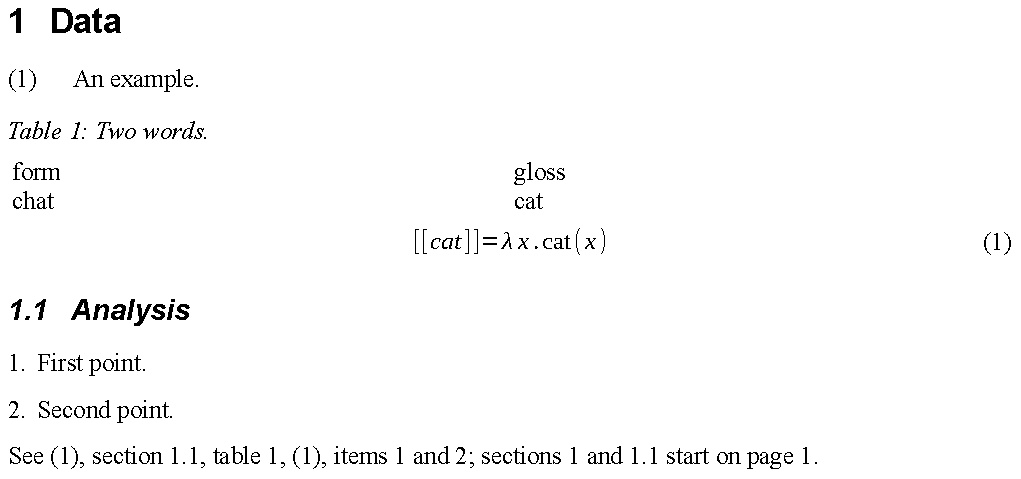
\includegraphics[width=0.85\linewidth]{figures/refs-odt}
\caption{Headings, a caption, an equation and a list, numbered as \LaTeX{}
numbers them, and references to each, all of them fields but the
equation's. The source is
\file{figures/src/refs.tex}; \LaTeX{} prints the same last line.}
\label{fig:refs}
\end{figure}

What a reference prints was measured against \LaTeX{} with \pkg{hyperref}
and \pkg{cleveref}, for every command and every kind of target. A
reference prints what \LaTeX{} prints, with the few exceptions in
section~\ref{sec:xref-diff}.

\subsection{What each reference becomes}

\begin{longtable}{@{}p{3.3cm} p{4.6cm} p{5.3cm}@{}}
\toprule
\textbf{Target} & \textbf{\file{.odt}} & \textbf{\file{.docx}}\\
\midrule
\endhead
example & \texttt{text:sequence-ref} to \texttt{NumEx} & \texttt{REF} to a bookmark around the \texttt{SEQ}\\
section & \texttt{text:bookmark-ref}, format \emph{chapter} & \texttt{REF \textbackslash w}, the number in full context\\
section title (\cs{nameref}) & \texttt{text:bookmark-ref}, format \emph{text} & \texttt{REF}, the bookmarked title\\
table, figure & \texttt{text:sequence-ref} to the caption's sequence & \texttt{REF} to a bookmark around the caption's \texttt{SEQ}\\
footnote & \texttt{text:note-ref} & \texttt{NOTEREF}\\
list item & one \texttt{text:bookmark-ref} per level, format \emph{number-no-superior} & one \texttt{REF \textbackslash n} per level\\
equation & text & text\\
page & the reference's \emph{page} format & \texttt{PAGEREF}\\
\bottomrule
\end{longtable}

Each field is written with the value \LaTeX{} prints already in it. That is
what a reader that never updates fields shows, and it is right, pages
included (section~\ref{sec:pages}).

\subsection{Examples}\label{sec:xref-ex}

\cs{ref}\{x\} prints ``(3)'', \cs{pref}\{x\} the bare ``3'', and a
sub-example ``(3a)''. The brackets are the document's \cs{ExLBr} and
\cs{ExRBr}. References may point forward, and they may appear inside
examples. The relative references \cs{Next}, \cs{Last}, \cs{NNext},
\cs{LLast} and their \texttt{p} forms are resolved by position, as
\pkg{linguexx} resolves them; inside an example \cs{Last} is the example
itself. Ranges, \cs{refrange} and \cs{prefrange}, print ``(3a--c)'' or
``(1--3a)'' with a live field at each end. \cs{cref} to an example prints
``(1)'', as \pkg{linguexx} sets it up. A label that no example carries prints
``??'', with a warning.

A reference to an example with a \emph{custom} label, \cs{ex.[(7)]}, prints
the label, ``(7)'' or ``(5a)'', as \pkg{linguexx}~1.4 does. It is text, not a
field: a custom label is not a counter, and nothing renumbers it.

\subsection{Sections and the appendix}\label{sec:sections}

The converter numbers the headings, because pandoc does not: \cs{section},
\cs{subsection} and \cs{subsubsection} as ``1'', ``1.1'', ``1.1.1'', by the
word processor's outline numbering, so they renumber when a section is moved.
A \cs{section*} gets no number and does not advance the count. A reference to
it, or to a \cs{paragraph}, prints the last number set before it, as \LaTeX{}
does.

\begin{center}\small
\begin{tabular}{@{}l l@{}}
\toprule
\textbf{Command} & \textbf{Prints}\\
\midrule
\cs{ref}\{s\} & 1.1\\
\cs{cref}\{s\}, \cs{Cref}\{s\} & section 1.1, Section 1.1\\
\cs{autoref}\{s\} & subsection 1.1 (the name follows the level)\\
\cs{nameref}\{s\} & the heading's title\\
\cs{pageref}\{s\}, \cs{cpageref}\{s\} & 3, page 3\\
\bottomrule
\end{tabular}
\end{center}

After \cs{appendix} the sections are lettered, ``A'', ``A.1'', in the headings
and in every reference to them. \cs{autoref} says ``Appendix A'' in the
document's language. Pandoc drops \cs{appendix} without a trace, so the
converter marks its place before pandoc reads the document. The appendix's
headings take a numbering of their own: a list in Writer, a second numbering
definition in Word.

The converter's heading numbering replaces any that a \opt{--reference-doc}
defines.

\subsection{Tables, figures and footnotes}

Pandoc writes a caption without a number. The converter numbers it as \LaTeX{}
does, ``Table~1: A table.'', with a live sequence for tables and another for
figures. Only a float with a \cs{caption} is counted, as only \cs{caption}
advances \LaTeX{}'s counter. \cs{ref} prints ``1'', \cs{cref} ``table~1'' or
``fig.~1'', \cs{autoref} ``Table~1'', and \cs{nameref} the caption without its
final full stop.

A reference to a footnote points at the note's mark in the text and shows its
number: ``footnote~2''. A footnote inside an example is a real footnote, in
both formats, and is counted with the rest. A \cs{label} inside a footnote
belongs to the footnote, as in \LaTeX, even when the footnote is inside an
example or a list item.

\subsection{Lists}

The converter numbers an \texttt{enumerate} as the \texttt{article} class
does, ``1.'', ``(a)'', ``i.'', ``A.'' by depth, from its start number (so
\cs{setcounter}\{enumi\}\{4\} gives ``5.''). A list whose style its source
names --- the \pkg{enumerate} package's \texttt{[(i)]} --- keeps that style.

A reference to an item is a field per level, on the item and each of its
parents: ``3'', ``2(b)i''. Pandoc writes a nested list as a list of its own,
so no word processor's ``number in context'' knows the parents. \cs{cref}
prints ``item~3'', and \cs{nameref} the title of the section the item is in,
as \LaTeX{} does.

\subsection{Equations}\label{sec:equations}

Pandoc writes display equations with no number. The converter numbers them as
\pkg{amsmath} does, and sets each number flush right beside its equation.
The paragraph style \sty{LxEquation} has a centre and a right tab stop, which
is how Writer and Word number their own equations.
\begin{itemize}[nosep]
\item \texttt{equation} and \texttt{multline}: one number;
\item \texttt{align}, \texttt{gather}, \texttt{alignat}, \texttt{flalign},
  \texttt{eqnarray}: one number per row, none for a row with \cs{nonumber}
  or \cs{notag};
\item \cs{tag}\{x\}: ``(x)'', not advancing the count;
\item starred environments, \cs{[}\,\ldots\,\cs{]} and \texttt{displaymath}: none;
\item \cs{numberwithin}\{equation\}\{section\} (or \cs{counterwithin}):
  ``(1.2)'', ``(A.1)'', starting again at each section.
\end{itemize}
An \texttt{align} with several numbers is set one row per line, so that each
number stands beside its row; its \texttt{\&} alignment is lost there. One
with a single number stays whole.

A reference to an equation is \textbf{text}: ``1'', \cs{eqref} ``(1)'',
\cs{cref} ``eq.~(1)'', \cs{Cref} ``Equation~(1)'', \cs{autoref} ``Equation~1''.
Neither the numbers nor the references follow a renumbering in the word
processor. \cs{nameref} is the live title of the section the equation is in,
and \cs{pageref} a live page.

\subsection{Several labels: \cs{cref} lists and ranges}

\cs{cref} and \cs{Cref} with several labels, and \cs{crefrange}, print what
\pkg{cleveref} prints:
\begin{itemize}[nosep]
\item the labels go in groups by kind, in the order each kind first comes:
  \cs{cref}\{s1,t1,s2\} is ``sections 1 and 2 and table 1'';
\item within a group they are sorted, a repeat is dropped, and a run of three
  or more consecutive numbers becomes a range: ``sections 1 to 3 and 5'';
\item groups are joined as \pkg{cleveref} joins them: ``section~1, table~1,
  and eq.~(1)'', with or without the last comma depending on the language;
\item a group of several takes the plural name, and \cs{Cref} capitalises the
  first group only.
\end{itemize}
Each number is a field of its own. The grouping, sorting and ranges are
worked out at conversion time; they stay as they are when the numbers change
later.

\subsection{Pages}\label{sec:pages}

A page is known only once the document is laid out, and a converter does not
lay out. So when LibreOffice and \texttt{pdfinfo} are installed, the converted
file is laid out once: it is exported to PDF with its bookmarks as named
destinations, and each page field gets the page its bookmark lands on. Word and
LibreOffice still compute their own when they update the fields. A reader that
never updates them, such as OnlyOffice with a \file{.docx}, shows LibreOffice's page.

Without LibreOffice a page field shows ``?'' until the word processor updates
it, and the run says so once. In an \file{.odt}, a page reference to an
\emph{example} or a \emph{footnote} always shows ``?'' until then, since
neither is a bookmark the layout can report; LibreOffice computes it when it
loads the file.

\subsection{The language of the names}\label{sec:names}

``section~1'' is ``Abschnitt~1'' in a German document, and a caption's
``Table~1:'' is ``Tableau''---or rather ``Table~1~--'' in French. Three packages
supply these names, and each has its own idea of the document's language.
The converter follows them as \LaTeX{} does:

\begin{center}\small
\begin{tabular}{@{}p{4.2cm} p{8.8cm}@{}}
\toprule
\textbf{Names} & \textbf{Follow}\\
\midrule
\cs{cref}, \cs{Cref}, \cs{cpageref} & the language given to \pkg{cleveref} as an
  option, or to the class. \emph{Not} \pkg{babel}'s option alone: with
  \texttt{\cs{usepackage}[ngerman]\{babel\}} and a bare
  \texttt{\cs{usepackage}\{cleveref\}}, \LaTeX{} prints ``section~1'', and so
  does the converter.\\
\cs{autoref} & \pkg{babel}'s main language. Under \pkg{polyglossia},
  hyperref's names stay English.\\
captions & \pkg{babel}'s main language, or \pkg{polyglossia}'s
  (\cs{setmainlanguage}), which do not always agree: ``Table 1 --'' under
  babel, ``Tab. 1 :'' under polyglossia, in French.\\
\bottomrule
\end{tabular}
\end{center}

The names are measured, not translated: \file{tools/measure\_names.py}
compiles a probe document in each language and loading style, reads the
names off the PDF, and checks the table the converter carries. English,
French, German, Spanish, Italian, Portuguese and Dutch are measured. Another
language prints English, and the run says so.

\subsection{Differences from \LaTeX}\label{sec:xref-diff}

\begin{itemize}
\item A reference to a list item whose label has parentheses keeps them:
  ``2(b)'' where \LaTeX{} prints ``2b'', ``(ii)'' for the \pkg{enumerate}
  package's \texttt{[(i)]} where \LaTeX{} prints ``ii''. Neither word
  processor has a reference format that drops them.
\item References to equations are text, as decided for this project; they do
  not follow a renumbering.
\item \cs{cpageref} with several labels on one page prints ``pages 1 and 1''
  where \pkg{cleveref} merges them into ``page 1'': the pages are known only
  after the phrase is written.
\item A \texttt{table} environment with no \texttt{tabular} in it, an image
  in a table float, is dropped by pandoc along with its caption and label. A
  reference to it prints ``??''.
\item \texttt{enumitem}'s \texttt{label=} is not read; such a list is
  numbered as the article default.
\end{itemize}

% ============================================================================
\section{The rest of the document}\label{sec:rest}

\subsection{Citations}

\pkg{natbib} and \pkg{biblatex} citations are resolved with pandoc's
\texttt{citeproc}, and a reference list is added at the end. The document
already declares its bibliography with \cs{addbibresource} or
\cs{bibliography}, and that is what is used:
\begin{code}
linguexx2odt paper.tex                           # the .bib the document names
linguexx2odt paper.tex --bibliography refs.bib   # or another
linguexx2odt paper.tex --csl unified-style-sheet.csl
\end{code}
\cs{citet} comes out author-in-text, \cs{citep} parenthetical, and an optional
locator survives: \cs{citep}[786]\{fruyt2011\} gives ``Fruyt 2011, 786''.
Pandoc has a single author-in-text mode, so \cs{citealt}, \cs{citeauthor}
and \cs{citeyear} all print ``Author (Year)''; the run says how many there
are of each.

If no \file{.bib} is found, the keys are printed, ``[vincent1982]'', and the
run says so. A citation nothing resolved would otherwise disappear from the
sentence.

\subsection{Included files and macros}

\cs{input}, \cs{include} and \cs{includeonly} are read and converted as part
of the document, examples and references included. A file is looked for in
the main document's directory, then through \texttt{kpsewhich}, so
\texttt{TEXINPUTS} and \file{\textasciitilde/texmf} are searched too. A file
the \TeX{} distribution ships, such as \cs{input}\{glyphtounicode\}, is engine
configuration: it is found and not read. Warnings name the file and line they
are about.

The document's own macros (\cs{newcommand}, \cs{renewcommand},
\cs{providecommand}, \cs{def}) are expanded inside examples, arguments and
optional defaults included. \cs{NewDocumentCommand} and \cs{def} with
delimited parameters are not read.

\subsection{What pandoc deletes}

Anything the converter does not handle goes to pandoc. What pandoc cannot
convert either is deleted from the output, and the run names each command or
environment it deleted, with a count. Commands that set no text --- spacing,
page breaks, font sizes --- are deleted without a word.

% ============================================================================
\section{Writing examples in the word processor}\label{sec:inside}

A converted document often goes on growing in the word processor. Three
companions build the converter's examples there: the same table, the same
named styles, the same \texttt{NumEx} numbers. A converted example and a
hand-built one are therefore the same kind of object, and both renumber
together.

\subsection{The Writer macro}

Type an example as lines, select them, and run \menu{Typeset example}:
\begin{code}
Esto es un ejemplo glosado
this is a example glossed
'This is a glossed example.'
\end{code}
The result is a numbered, aligned example. The macro does two things the
converter cannot: it \emph{measures} the real font instead of estimating, and
it reads the actual page instead of trusting \opt{--text-width}.
\begin{itemize}[nosep]
\item Sub-examples typed \texttt{a.}, \texttt{b.}; a leading \texttt{*} or
  \texttt{?} for a judgment; \texttt{\{braces\}} for one column;
  \cs{exannot}\{\ldots\} for a label.
\item \menu{Typeset numbered tree} and \menu{Typeset unnumbered tree} draw
  syntax trees from bracket notation, \texttt{[DP [D the] [NP [N tree]]]},
  with roofs and movement arrows.
\item \menu{Untypeset example} gives an example back as the lines it was
  built from, with its number at their head. Edit them and typeset again,
  and it is the same example with the same number, so no reference breaks.
\item \menu{Example layout\ldots} sets the indents and the spacing, which
  belong to the document.
\end{itemize}
Install it as a LibreOffice extension: add \file{linguexx-0.1.0.oxt} (from
the project's latest release, or \texttt{python3 tools/build\_oxt.py}) in
\menu{Tools \textrightarrow{} Extension Manager}. \file{docs/macro.md}
describes it in full.

\subsection{The Word and OnlyOffice add-ins}

Two add-ins do in Word and OnlyOffice what the macro does in Writer:
\menu{Typeset selection}, \menu{Typeset tree}, \menu{Untypeset example},
\menu{Example layout}, and \menu{Insert reference\ldots}, which lists the
document's examples and inserts a live reference, ``(3)'' or the bare
``3''.
\begin{itemize}
\item \textbf{OnlyOffice}: install \file{linguexx-onlyoffice.plugin} from
  the latest release (or \texttt{make onlyoffice}) through \menu{Plugins
  \textrightarrow{} Plugin Manager}. Renumbering is immediate.
\item \textbf{Word}: the add-in has to be served over HTTPS; for now that is
  a server on your own machine, \texttt{python3 tools/serve\_addin.py}. Then
  upload \file{addin/word/manifest.xml} under \menu{Home \textrightarrow{}
  Add-ins \textrightarrow{} My Add-ins}. Word for the desktop renumbers with
  \texttt{Ctrl+A}, \texttt{F9}. Word on the web never renumbers fields;
  the pane says which numbers are stale.
\end{itemize}

% ============================================================================
\section{Back to \LaTeX}\label{sec:back}

A document that went to Word or Writer and was edited there can come back:
\begin{code}
docx2linguexx paper.docx -o paper.tex
odt2linguexx  paper.odt  -o paper.tex
\end{code}
Every example table becomes a \pkg{linguexx} example again: tiers, braced
groups, judgments, sub-examples on both levels, the translation and
\cs{exannot}. Every reference to an example becomes \cs{ref} or \cs{pref}
with a label. The rest is pandoc's \LaTeX{} writer, with
\texttt{\cs{usepackage}[lazy]\{linguexx\}} added.

It reads the paragraph styles and fields that the converter, the macro and the
add-ins write. An example typed by hand with tabs or spaces is not recognised
and comes back as prose or as a table. An \file{.odt} is first saved as
\file{.docx} by LibreOffice, which therefore has to be installed, because
pandoc's own ODT reader drops the text of every cross-reference.

The way back's test is the way forward: every test document, and every
document in \pkg{linguexx}'s own test suite, is converted to \file{.docx} and
back, and must give the same examples, cell for cell.

\begin{itemize}
\item Labels are generated (\texttt{ex:1}, \texttt{ex:2a}): the word processor
  never had the author's. Only an example something refers to gets one.
\item Drawn trees come back as \pkg{forest} trees.
\item The layout is not read back: \pkg{linguexx} sets its own widths and
  bands.
\end{itemize}

% ============================================================================
\section{Limits}\label{sec:limits}

The converter warns about everything in this list.

\begin{longtable}{@{}p{4.6cm} p{8.6cm}@{}}
\toprule
\textbf{Construct} & \textbf{What happens}\\
\midrule
\endhead
\cs{ex.} inside \texttt{itemize}, \texttt{enumerate} or a footnote & not
  converted: the example's text stays as ordinary unnumbered text\\
\cs{altn}, \cs{altg} & not supported: neither format can draw a stack of
  alternatives. Deleted with their arguments (printed as source inside an
  example in a \file{.docx})\\
a list or table inside an example & not supported: an example table cannot
  hold a second layout\\
\cs{mvto}, \cs{mvfrom} & the arrows are not drawn; the words stay\\
\pkg{forest}, \cs{Tree} trees & kept as bracket notation, for the macro or
  the add-ins to draw\\
\cs{exsource} & set at the end of the example, not flush right\\
\cs{GlossTransSide} & the translation is set below, not beside: a side
  column has no defined behaviour when an example splits into bands\\
\texttt{[phantomalign]} & judgment marks get a column of their own\\
\cs{GlossTierFont}, \cs{SetLeipzig}, \cs{DeclareJudgment} & the styles and
  the literal marks are used\\
a reference to a sub-sub-example & printed without its sub-example's letter,
  ``(1i)'' for ``(1b-i)''\\
\texttt{[langsci]}'s \cs{ea}\,\ldots\,\cs{z}, \pkg{gb4e}'s \texttt{exe} &
  out of scope: the first degrades to unnumbered text, the second is deleted\\
\texttt{[legacy]} mode & out of scope\\
math inside an example & handed to pandoc, which may not keep it\\
\bottomrule
\end{longtable}

\noindent The cross-references' own differences are in
section~\ref{sec:xref-diff}.

% ============================================================================
\section{Troubleshooting}\label{sec:trouble}

\begin{description}[style=nextline,leftmargin=1.5em]
\item[The numbers did not change after I inserted an example.]
  Update the fields: \texttt{F9} in Writer, \texttt{Ctrl+A} then \texttt{F9}
  in Word for the desktop. Word on the web does not update fields.
\item[OnlyOffice shows an old number.] OnlyOffice shows a field's stored
  value. The converter stores the right one; an edit made since is shown once
  the field is refreshed.
\item[A page reference shows ``?''.] The conversion had no LibreOffice or
  \texttt{pdfinfo} to lay the document out. The word processor fills it in
  when it updates the fields.
\item[A column is too narrow or too wide.] The widths are estimated
  (section~\ref{sec:widths}). Check \opt{--font} and \opt{--font-pt}, drag
  the column in the word processor, or rebuild the example with the macro,
  which measures.
\item[\texttt{python3 -m linguexx2odt} finds no module.] Run it with
  \texttt{PYTHONPATH=src} from a checkout, or install the package.
\item[A test or conversion that renders seems to hang.] Suspect OpenCL:
  LibreOffice probes it at startup, and a broken entry in
  \file{/etc/OpenCL/vendors} hangs the probe. \texttt{SAL\_DISABLE\_OPENCL=1}
  works around it.
\end{description}

% ============================================================================
\section{For developers}\label{sec:dev}

\begin{code}
make check            # lint and the test suite: what CI runs
make test             # the suite alone
make js-test          # the add-ins' suite (Node 22 or later)
make onlyoffice-test  # the OnlyOffice plugin, in Document Builder
make manual           # this manual
\end{code}

The end-to-end tests build real documents, render them with LibreOffice and
measure the PDF. They check that numbers evaluate (with every stored value
corrupted first, so that echoing cannot pass), that references resolve, that
glosses sit under their words, that judgment marks do not shift the text and
that nothing runs into the margin. They need \texttt{pandoc}, \texttt{soffice}
and \texttt{pdftotext}. A missing one is a \emph{failure}, not a skip, so that
a contributor without LibreOffice does not see green and ship;
\texttt{LINGUEXX2ODT\_ALLOW\_MISSING=1} runs a partial suite on purpose.

Several tables in the converter are measurements, each with a tool that checks
it:
\begin{description}[style=sameline,leftmargin=1.5em,nosep]
\item[\file{tools/measure\_advances.py}] the per-character widths of the
  Times-metric faces, against the font;
\item[\file{tools/measure\_names.py}] the names of references and captions,
  per language, against \LaTeX{};
\item[\file{tools/validate\_docx.py}] a \file{.docx} against the ECMA-376
  schemas;
\item[\file{tools/sync\_macro.py}] the constants the converter shares with the
  macro and the add-ins.
\end{description}
\file{notes/findings.md} records what was measured and why each design
decision was taken; the \file{plan-*.md} files are the work orders, with what
was tested and what remains. The repository's layout is described at the end
of \file{README.md}.

% ============================================================================
\section*{Licence}
\addcontentsline{toc}{section}{Licence}

Copyright \textcopyright{} 2026 Gerhard Schaden. This program is free
software: you can redistribute it and/or modify it under the terms of the GNU
General Public License as published by the Free Software Foundation, either
version~3 of the License, or (at your option) any later version.

\pkg{linguexx} itself is under the \LaTeX{} Project Public License~1.3c, a
different licence for a different kind of work. The converter only reads
\pkg{linguexx} documents; it includes none of the package's code.

\end{document}
